\documentclass[dvips,11pt]{article}

% Any percent sign marks a comment to the end of the line

% Every latex document starts with a documentclass declaration like this
% The option dvips allows for graphics, 12pt is the font size, and article
%   is the style

\usepackage[letterpaper, margin=1in]{geometry}

\usepackage[pdftex]{graphicx}
\usepackage{url}
\usepackage[pdftex]{xcolor}
\usepackage{amsmath}
\usepackage{enumitem}
\usepackage{tabularx}

\usepackage{fancyhdr}
\pagestyle{fancy}
\fancyhf{}
\lfoot{2017 CFA Narrative 12924}
\rfoot{Page \thepage\ of \pageref{LastPage}}

\renewcommand{\headrulewidth}{0pt}
\renewcommand{\footrulewidth}{0.5pt}

\newcommand{\unc}[1]
{ \delta #1 }

\newcommand{\uncsq}[1]
{ \left(\unc{#1}\right)^2 }

\newcommand{\uncratio}[1]
{ \left(\frac{\unc{#1}}{#1}\right) }

\newcommand{\uncratiosq}[1]
{ \uncratio{#1}^2 }

\newcommand{\uncvector}[1]
{ \left[ \begin{array}{c} #1 \\ \delta #1 \end{array} \right] }

\newcommand{\comment}[1]
{{\bfseries \color{red} #1}}

\makeatletter
\renewcommand\section{\@startsection {section}{1}{\z@}%
                                   {-2.0ex \@plus -1ex \@minus -.2ex}%
                                   {2.3ex \@plus.2ex}%
                                   {\normalfont\bfseries}}% from \Large
\renewcommand\subsection{\@startsection{subsection}{2}{\z@}%
                                     {-2.0ex\@plus -1ex \@minus -.2ex}%
                                     {1.5ex \@plus .2ex}%
                                     {\normalfont\bfseries}}% from \large
\renewcommand\subsubsection{\@startsection{subsubsection}{3}{\z@}%
                                     {-2.0ex\@plus -1ex \@minus -.2ex}%
                                     {1.5ex \@plus .2ex}%
                                     {\normalfont\bfseries}}% from \normalsize
\makeatother


%----------------------------------------------------------------------------------------
%	DOCUMENT INFORMATION
%----------------------------------------------------------------------------------------
\begin{document}
\begin{centering}
  Application Narrative for DE-FOA-0001515\\
  \textbf{\large Sensitivity of Fuel Cycle Decision Making to 
  Modeling Choices and Data Uncertainty}\\
  2016 CFA Narrative 12924\\
\end{centering}
\vspace{1em}

\noindent\textbf{Technical Workscope Identifier:} #TBD \hspace{1.5in}
\textbf{Time Frame:} 2 years

\section{Introduction \& Proposed Scope}
Nuclear fuel cycle simulation tools can have a large scope of application, from
the study of the behavior of a particular type of fuel or reactor inside an
existing nuclear fleet to the prospective analysis of a complete nuclear
transition.  Each use case requires a specific level of confidence, which are up
to now very poorly assessed, if assessed at all.  Indeed, the only existing way
to develop confidence in any fuel cycle calculation/tool, is to compare with
other similar tools or historical data.  For the former, the conclusion if often
a list of why the different software gave different results with no conclusion
on the precision of any.  The latter only allows validation of existing concepts
and has no impact on calculations based on the use of new concepts.

The aim of this project is to add error propagation capability to the Cyclus
fuel cycle simulator\cite{Cyclus_paper}. Given the use case of predicting the
evolution of a large industrial enterprise in an uncertain future, nuclear fuel
cycle simulations are generally based on approximate models and uncertain input
data.  Since strict validation is largely considered to be impractical, such
simulations are seen as indications of trends in future behavior rather than
predictions of that behavior. Nevertheless, it would be valuable to be able to
place some confidence bounds on those indications, both to assess the robustness
of conclusions that derive from those indications and to provide information
about the sensitivity of those conclusions to the uncertain data and algorithms.
Having a broad distribution for each metric calculated in a fuel cycle
simulation instead of unique values will allow a better comparison between
different fuel cycle scenarios.  Moreover for some critical use cases, it could
be extremely valuable to add some degree of confidence on the results of the
simulation.  This could result in confidence in the use of the tool for such
uses, and confidence in the conclusions that follow from those results.

This project will extend the Cyclus concept of resources to include error
information and then develop a number of archetypes that can perform operations
to propagate that error in a manner that is consistent with the physical models
of the archetype.  The ultimate calculation of fuel cycle performance metrics
will also need to be updated in order to represent final results as
distributions rather than single values.  The primary outcome will a
demonstration of, and a framework for, performing error propagation, but not a
comprehensive implementation of error propagation for all models across all
archetypes.  Other researchers will then be able to extend this capability for
additional archetypes, whether pre-existing or newly developed.

\section{Logical Path to Work Accomplishment}
The goal of this project is to add optional extensions to Cyclus that will allow
an assessment of the error as it propagates through a fuel cycle.  Four tasks
are identified to accomplish this goal.




\section{Relevance of Proposed Research}


\begin{figure}[h!]
\centering
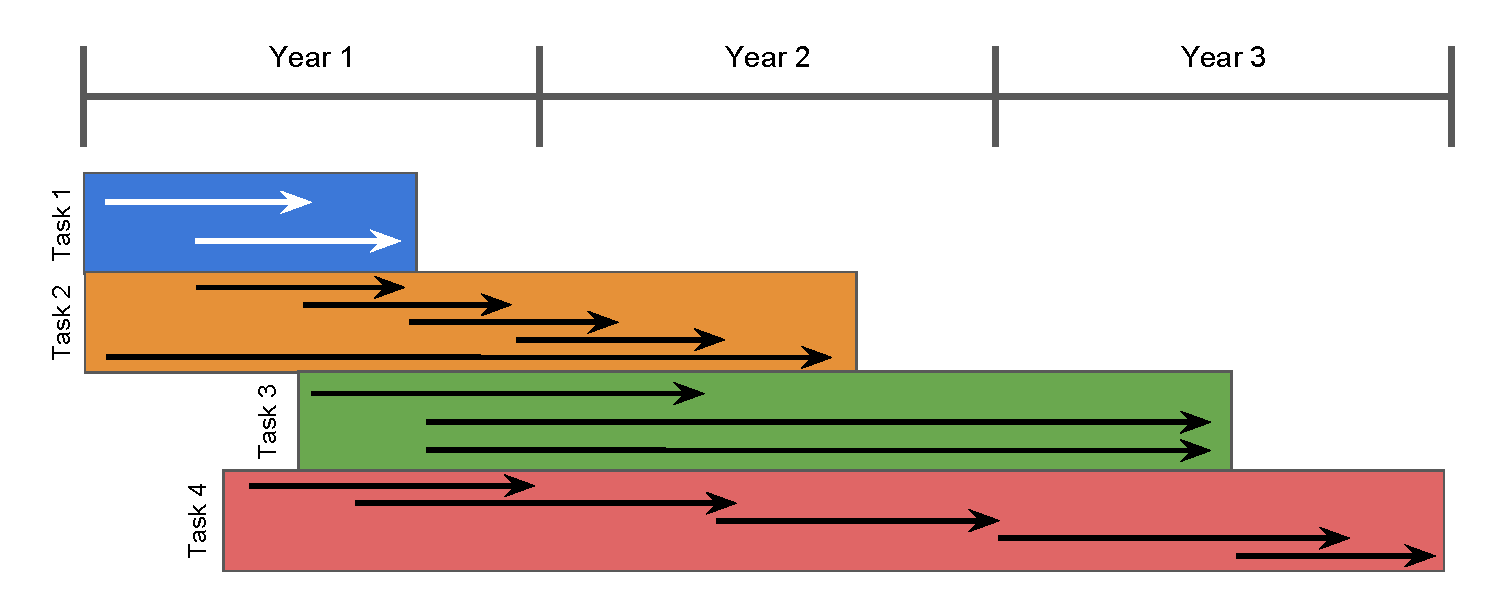
\includegraphics[width=\textwidth]	{timeline}
\caption{Preliminary schedule of the project indicating tasks and subtasks}
\label{fig:progression}
\end{figure}

\newpage
\noindent\textbf{TASK 1:}
\begin{itemize}[nosep]
\item subtask 1: 
\item subtask 2: 
\end{itemize}

\noindent\textbf{TASK 2:}
\begin{itemize}[nosep]
\item subtask 1: 
\item subtask 2: 
\item subtask 3: 
\item subtask 4: 
\item subtask 5: 
\end{itemize}

\noindent\textbf{TASK 3:}
\begin{itemize}[nosep]
\item subtask 1:
\item subtask 2:
\item subtask 3:
\end{itemize}
 
\noindent\textbf{TASK 4:}
\begin{itemize}[nosep]
\item subtask 1:
\item subtask 2:
\item subtask 3:
\item subtask 4:
\item subtask 5:
\end{itemize}

\begin{table}[h!]
\caption{List of major milestones and deliverables}
\begin{tabularx}{
\textwidth}{|X|c|l|}\hline
 \textbf{Milestone}       & 
     \textbf{Date}$^*$&
     \textbf{Deliverable} \\\hline
 Completion and testing of basic material operations      &   
     12                         & 
     Report on Tasks 1 \& 4.1   \\\hline
 Demonstration of uncertainty propagation with simple archetypes  &   
     18       & 
     Report on Tasks 2.1, 2.2 \& 4.2 \\\hline
 Demonstration of uncertainty propagation with extended Cycamore archetypes &
     24       &
     Report on Tasks 2.3, 2.4, 2.5 \& 4.3 \\\hline
 Demonstration of uncertainty propagation with CLASS-based archetypes &
     33       &
     Report on Tasks 3 \& 4.4 \\\hline
 Demonstration of uncertainty propagation on representative fuel cycle transitions &
     36       &
     Final report\\\hline
\end{tabularx}
{\footnotesize $^*$ all dates are given in months from project start}
\end{table}

\section{Facilities}

Most of the development work for this project will be carried out on desktop
workstation or laptop computers with free and open source software and software
libraries. Desktop computing capabilities are available to the investigators;
where additional computing platforms are required (for instance, for graduate
students working on the project), funding for them is requested.

Where larger computational resources are required, the lead institution
maintains a variety of centrally-supported computing resources, including a
large pool of distributed computing resources and a growing tightly coupled high
performance computing resource. The distributed computing pool gives researchers
access to over 10,000 computing cores, and seamless capability of reaching the
nationally distributed Open Science Grid. Combined, these resources routinely
provide researchers with approximately 300,000 CPU hours per day. If the
algorithms favor a high performance computing mode, the cluster at has over 3000
cores with 30 TB of RAM, connected with a 56 GB/s Infiniband backplane.

\section{Quality Assurance \& Software Development Process}

\textit{This project will comply with all Quality Assurance requirements, as
described on the NEUP website.}  

This work will follow the Cyclus development model.  We will employ a variety of
modern software project management tools: revision control, automated testing,
automated and manual documentation, bug tracking. Related projects at are
already managed under source code revision control system (git) that provides
detailed tracking of all changes to the code base. A test suite has been
developed and new tests will be added for each new capability. This test suite
will be automatically executed with each proposed change in the revision control
system to identify any flaws that may be introduced. Automated documentation
tools are used in the source code to create a detailed reference for the
interfaces and additional background documentation. Out-of-code detailed reports
and publications will supplement the information on each new capability.
Finally, a bug tracking system (GitHub issues) is deployed to help users and
developers to understand known issues and to track their resolution as a
developer community. As new capability is added, it will come under the same
quality assurance practices as described here for the existing capabilities.

%----------------------------------------------------------------------------------------
%	BIBLIOGRAPHY
%----------------------------------------------------------------------------------------

\bibliographystyle{narrative}

\bibliography{narrative}

%----------------------------------------------------------------------------------------

\label{LastPage}
\end{document}
